\documentclass[11pt]{article}
\usepackage[margin=18mm]{geometry}
\usepackage{graphicx,booktabs}
\begin{document}
\title{Ion and photon pulses per readout cell}
\author{NAUSICAA generated report}
\date{}\maketitle
\section*{Sample and assumptions}
The 1 mm Geant4 source samples contribute 8,000 events each. The same Fano-sampled primary pairs and event placement feed all branches. W = 21.90 eV, F = 0.150; electron lifetime = 15.0 ms, E/P = 3.0 kV/cm/bar, J = 0.010. All occupied cells and all events with pulses enter the distributions; no count cut is applied. Carriers were sampled directly into physical readout cells, with no diffusion-histogram truncation. No time-integrated pixel or SiPM charge enters these plots. The ion and photon ledgers are exact against their saved histories.
\section*{Ion pixel--frame pulses}
An ion pulse is one pixel--frame cell with positive ion count. The three ion grids use 2, 3 and 4 mm transverse pitch and 20, 30 and 40 ms frames, respectively, corresponding to 2, 3 and 4 mm along drift. Every event mean is its total ions divided by its number of occupied pixel--frame cells; the event maximum is the largest cell count.
\begin{center}\resizebox{\linewidth}{!}{\begin{tabular}{lllllllll}\toprule Species & Setting & Events & Occupied cells & Total signal & Mean of means & Median mean & Mean maximum & Median maximum\\\midrule
Double beta & 2 mm / 20 ms & 8,000 & 13,474,452 & 897,306,359 & 81.89 & 67.21 & 2,027.4 & 1,570.0\\
Double beta & 3 mm / 30 ms & 8,000 & 5,326,135 & 897,306,359 & 200.25 & 170.58 & 4,342.7 & 3,787.0\\
Double beta & 4 mm / 40 ms & 8,000 & 2,828,841 & 897,306,359 & 367.58 & 321.51 & 6,759.6 & 6,245.0\\
Single electrons & 2 mm / 20 ms & 8,000 & 16,024,040 & 897,244,198 & 69.01 & 55.72 & 1,881.9 & 1,461.0\\
Single electrons & 3 mm / 30 ms & 8,000 & 6,386,831 & 897,244,198 & 167.14 & 140.46 & 4,007.4 & 3,475.5\\
Single electrons & 4 mm / 40 ms & 8,000 & 3,412,957 & 897,244,198 & 304.33 & 264.11 & 6,236.0 & 5,722.0\\
\bottomrule\end{tabular}}\end{center}
\begin{center}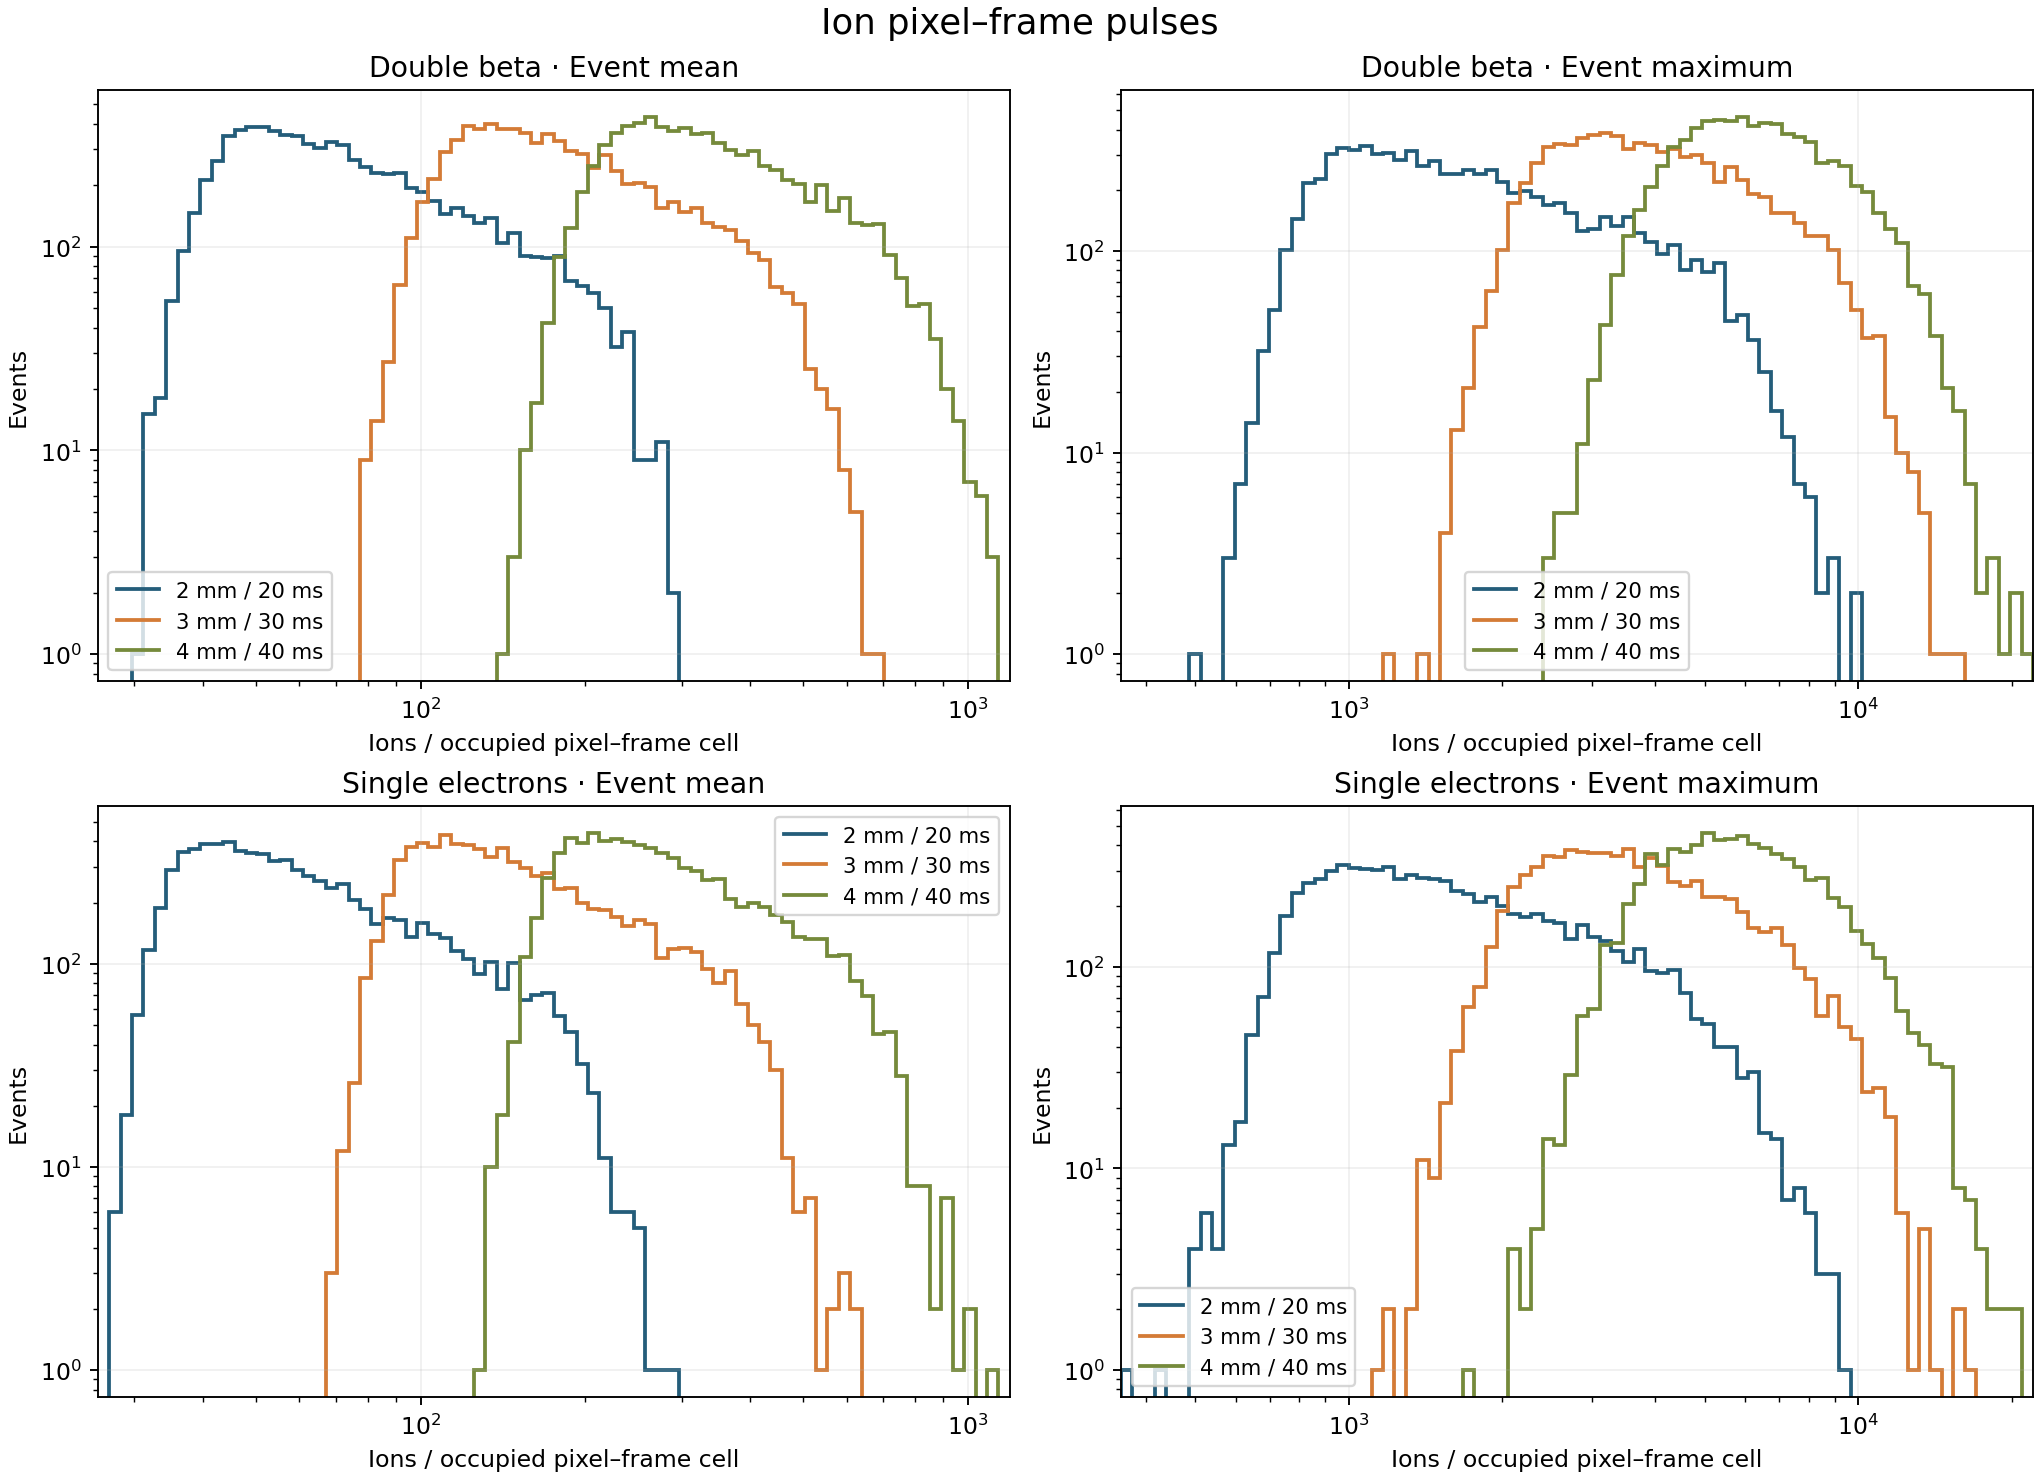
\includegraphics[width=\linewidth]{ions_mean_max.png}\end{center}
\clearpage\section*{Photon SiPM--bucket pulses}
A photon pulse is one SiPM--2 $\mu$s bucket with positive incident VUV photon count. Pure Xe and Xe--15\% He use the same 10 mm hole pitch and electron settings. Every event mean divides its total incident photons by its occupied SiPM--bucket count; the event maximum is the largest bucket count. These are incident photons before SiPM PDE and electronics.
\begin{center}\resizebox{\linewidth}{!}{\begin{tabular}{lllllllll}\toprule Species & Setting & Events & Occupied cells & Total signal & Mean of means & Median mean & Mean maximum & Median maximum\\\midrule
Double beta & Pure Xe & 8,000 & 7,709,774 & 381,687,642,280 & 79,472.22 & 50,385.34 & 1,302,701.2 & 844,057.0\\
Double beta & Xe--15\% He & 8,000 & 3,048,897 & 375,319,166,815 & 165,930.15 & 123,124.19 & 2,453,245.4 & 2,038,311.0\\
Single electrons & Pure Xe & 8,000 & 9,368,261 & 381,739,047,046 & 65,305.89 & 41,346.55 & 1,219,160.9 & 789,159.0\\
Single electrons & Xe--15\% He & 8,000 & 3,731,089 & 375,368,751,796 & 135,647.88 & 100,328.55 & 2,269,206.3 & 1,891,749.0\\
\bottomrule\end{tabular}}\end{center}
\begin{center}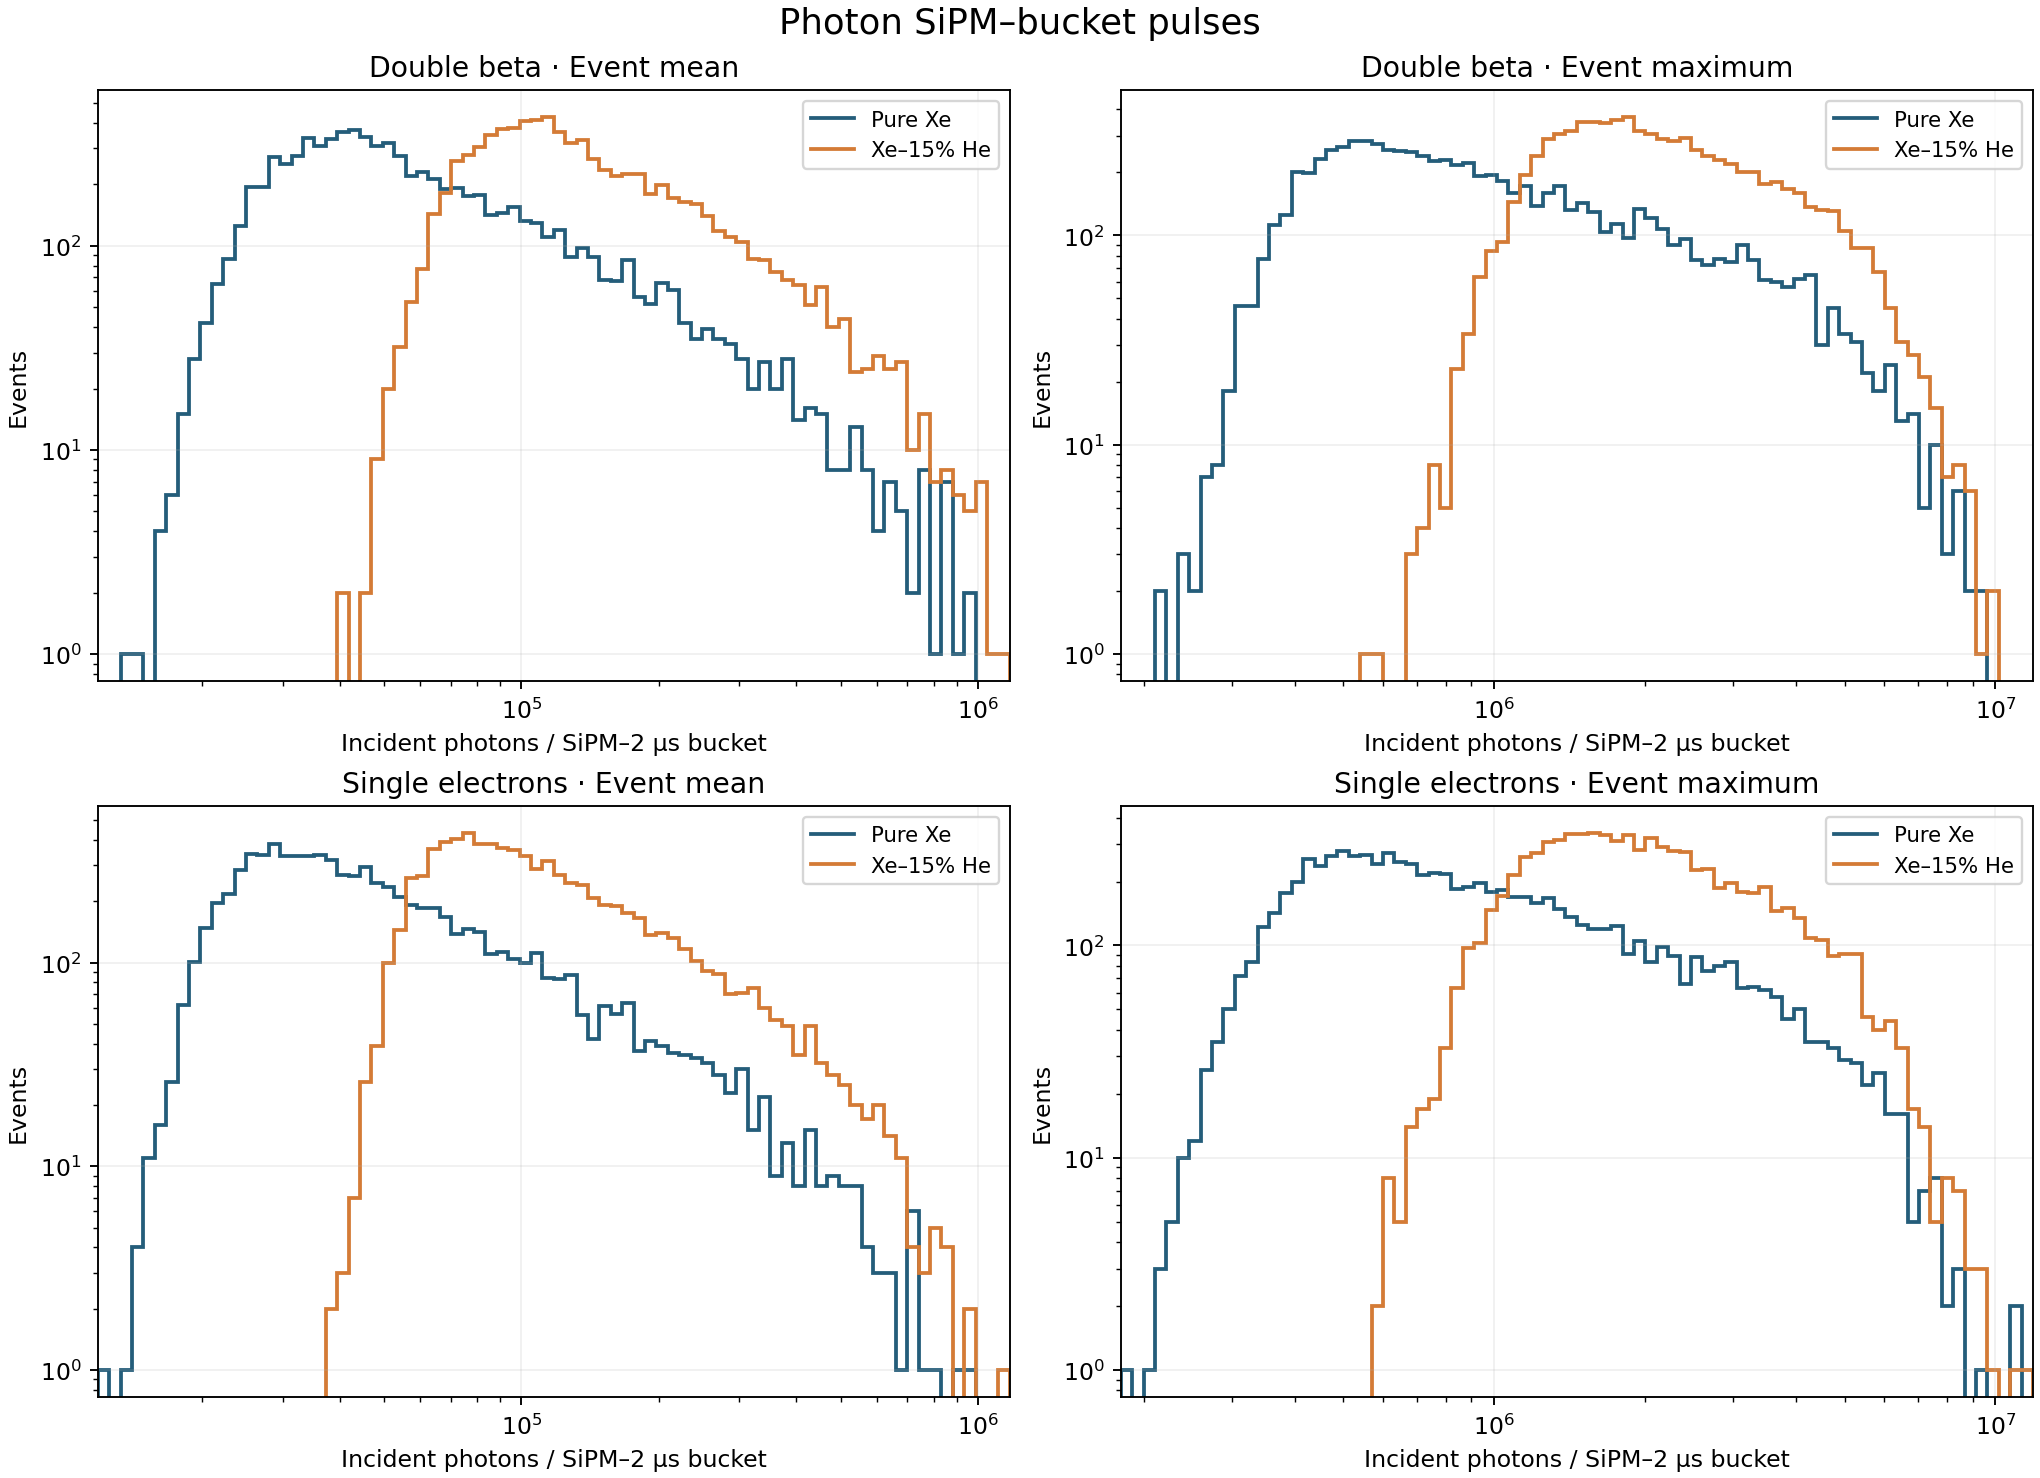
\includegraphics[width=\linewidth]{photons_mean_max.png}\end{center}
\section*{Provenance}
Numerical reduction: \texttt{readout\_pulses.h5}. Run ID: \texttt{238ddc5a75e0fd9b}. The HDF5 file preserves per-event values, histogram bins, resolved cards, source/code hashes and charge/light ledgers.
\end{document}
